\documentclass[letterpaper,12pt]{article}
\usepackage{array}
\usepackage{threeparttable}
\usepackage{geometry}
\geometry{letterpaper,tmargin=1in,bmargin=1in,lmargin=1.25in,rmargin=1.25in}
\usepackage{fancyhdr,lastpage}
\pagestyle{fancy}
\lhead{}
\chead{}
\rhead{}
\lfoot{}
\cfoot{}
\rfoot{\footnotesize\textsl{Page \thepage\ of \pageref{LastPage}}}
\renewcommand\headrulewidth{0pt}
\renewcommand\footrulewidth{0pt}
\usepackage[format=hang,font=normalsize,labelfont=bf]{caption}
\usepackage{listings}
\lstset{frame=single,
  language=Python,
  showstringspaces=false,
  columns=flexible,
  basicstyle={\small\ttfamily},
  numbers=none,
  breaklines=true,
  breakatwhitespace=true
  tabsize=3
}
\usepackage{amsmath}
\usepackage{amssymb}
\usepackage{amsthm}
\usepackage{harvard}
\usepackage{setspace}
\usepackage{float,color}
\usepackage[pdftex]{graphicx}
\usepackage{hyperref}
\hypersetup{colorlinks,linkcolor=red,urlcolor=blue}
\theoremstyle{definition}
\newtheorem{theorem}{Theorem}
\newtheorem{acknowledgement}[theorem]{Acknowledgement}
\newtheorem{algorithm}[theorem]{Algorithm}
\newtheorem{axiom}[theorem]{Axiom}
\newtheorem{case}[theorem]{Case}
\newtheorem{claim}[theorem]{Claim}
\newtheorem{conclusion}[theorem]{Conclusion}
\newtheorem{condition}[theorem]{Condition}
\newtheorem{conjecture}[theorem]{Conjecture}
\newtheorem{corollary}[theorem]{Corollary}
\newtheorem{criterion}[theorem]{Criterion}
\newtheorem{definition}[theorem]{Definition}
\newtheorem{derivation}{Derivation} % Number derivations on their own
\newtheorem{example}[theorem]{Example}
\newtheorem{exercise}[theorem]{Exercise}
\newtheorem{lemma}[theorem]{Lemma}
\newtheorem{notation}[theorem]{Notation}
\newtheorem{problem}[theorem]{Problem}
\newtheorem{proposition}{Proposition} % Number propositions on their own
\newtheorem{remark}[theorem]{Remark}
\newtheorem{solution}[theorem]{Solution}
\newtheorem{summary}[theorem]{Summary}
%\numberwithin{equation}{section}
\bibliographystyle{aer}
\newcommand\ve{\varepsilon}
\newcommand\boldline{\arrayrulewidth{1pt}\hline}


\begin{document}

\begin{flushleft}
  \textbf{\large{Problem Set \#2}} \\
  Perspectives on Computational Modeling \\
  MACS 30100, Dr. Evans \\
  HyungJin Cho
\end{flushleft}

\vspace{5mm}

\begin{enumerate}
  \textbf{Problem 1.}
\end {enumerate}
\begin{enumerate}
  \textbf{Part (a). Histogram}
\par
\begin{figure}[H]\centering\captionsetup{width=4.0in}
   \fbox{\resizebox{4.0in}{3.0in}{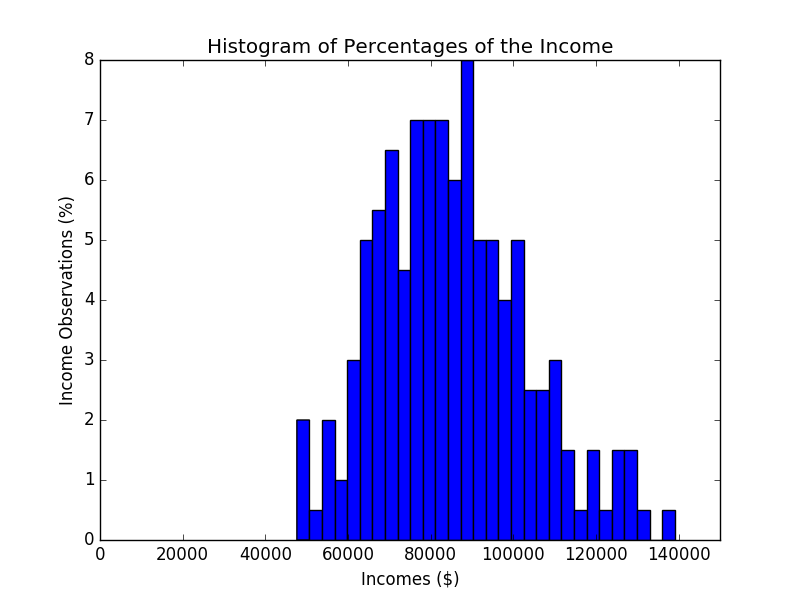
\includegraphics{./images/Figure_1(a).png}}}
\end{figure}
\par\bigskip
\end {enumerate}

\begin{enumerate}
  \textbf{Part (b). lognormal PDF}
\par
\begin{figure}[H]\centering\captionsetup{width=4.0in}
  \fbox{\resizebox{4.0in}{3.0in}{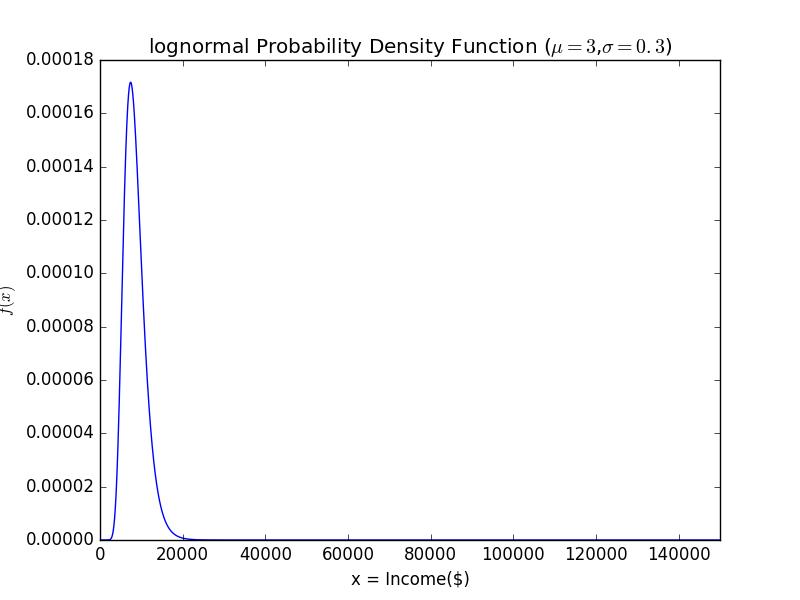
\includegraphics{./images/Figure_1(b).png}}}
\end{figure}
\par
Log-likelihood value = -8298.63695601
\par\bigskip
\end {enumerate}

\begin{enumerate}
  \textbf{Part (c). MLE}
\par
\begin{figure}[H]\centering\captionsetup{width=4.0in}
  \fbox{\resizebox{4.0in}{3.0in}{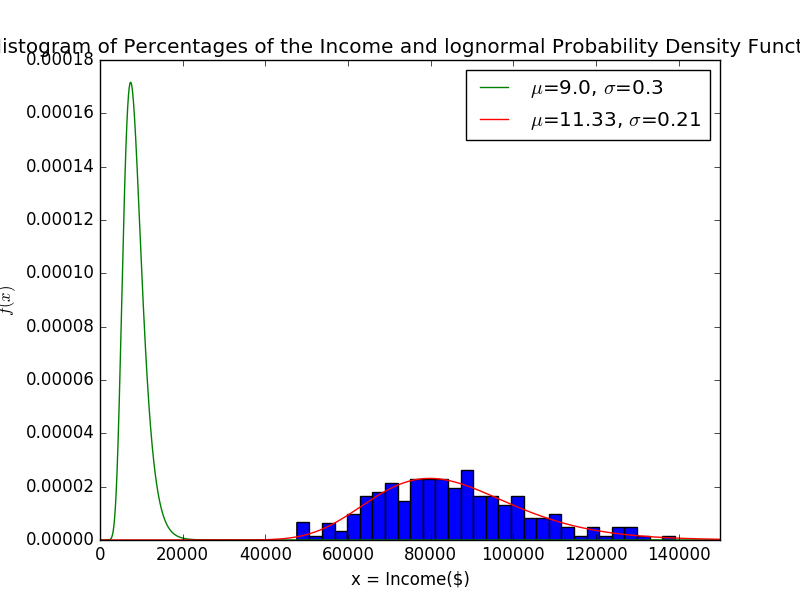
\includegraphics{./images/Figure_1(c).png}}}
\end{figure}
\par
$\mu$ MLE = 11.3314403326 \\
$\sigma$ MLE = 0.211674580757 \\
Log-likelihood Value = -2239.534744 \\
VCV =  [[ 1.  0.] \\
\hspace{12mm} [ 0.  1.]]
\par\bigskip
\end {enumerate}

\begin{enumerate}
  \textbf{Part (d). Chi-square Test}
\par\bigskip
$\chi^2$ of $H_{0}$ with 2 degrees of freedom p-value =  0.0
\par\bigskip
\end {enumerate}

\begin{enumerate}
  \textbf{Part (e). Inference}
\par\bigskip
The probability that you will earn more than \$100,000 is 19.561800210962077\%
\par
The probability that you will earn less than \$75,000 is 30.79396097251101\%
\par\bigskip
\end{enumerate}

\begin{enumerate}
  \textbf{Problem 2.}
\end {enumerate}

\begin{enumerate}
  \textbf{Part (a). MLE}
\par\bigskip
$\beta_{0}$ MLE = 0.259082991468 \\
$\beta_{1}$ MLE = 0.0141522942932 \\
$\beta_{2}$ MLE = 0.389203982613 \\
$\beta_{3}$ MLE = -0.0106002331579 \\
$\sigma^2$ MLE = 0.0159045883926 \\
Log-likelihood Value = 876.865053329 \\
VCV = [[ 1.  0.  0.  0.  0.] \\
\hspace{12mm}   [ 0.  1.  0.  0.  0.] \\
\hspace{12mm}   [ 0.  0.  1.  0.  0.] \\
\hspace{12mm}   [ 0.  0.  0.  1.  0.] \\
\hspace{12mm}   [ 0.  0.  0.  0.  1.]]
\par\bigskip
\end {enumerate}

\begin{enumerate}
  \textbf{Part (b). Chi-square Test}\par\bigskip
$\chi^2$ of $H_{0}$ with 5 degrees of freedom p-value =  0.0
\end {enumerate}

\end{document}
